\chapter{Analysis and solution}
\label{chap:AnalysisAndSolution}
\section{Data analysis}
\label{sec:DataAnalysis}
\subsection{Constructing buildings}
To construct the buildings, we would like to extract data for each building from the BAG data set. However, this data is incomplete. For each building, only a polygon is defined with geographical points. This polygon describes the contour and the exact position of a building. Thus the data contains no information on the height of the building or what kind of roof the building has. In order to determine the height of a building, we can however used the information stored in the residences of a building. For each residence the BAG-dataset contains the total surface area. Combining this with the total area of the surface geometry of a building, we are able to approximate the amount of floors of a building. To approximate the height of a building, we specify that each floor has a height of 2.5 meters. However, for some buildings, only some or no residences are specified, therefore some buildings will get an invalid height. Buildings with no residences will be constructed with an height of 2.5 meters.

Since the bag data set contains no information on the roof, all buildings will get a flat roof. To create the roof for a model cannot be done in a naïve way, since most of the models of the buildings are non-convex polygons. That is, not every point in the polygon is directly visible by all other points, and thus no direct edge can be constructed between two points without the possibility that this edge crosses an edge of the polygon. To produce the roof of a model, an ear slicing algorithm is used. The ear slicing algorithm is a well-known algorithm for triangulating a simple polygon \cite{Kajak11}. The algorithm iteratively locates an ear in the polygon and removes the ear. This process continues till the polygon is a triangle.

A vertex $p_i$ in a polygon is called an ear if the diagonal line between the neighbouring vertexes, $(p_{i-1}, p_{i+1})$, lies entirely within the polygon. That is, this diagonal $(p_{i-1}, p_{i+1}$ does not intersect with any other edge of the polygon. When an ear is found, it is removed from the polygon and the diagonal $(p_{i-1}, p_{i+1})$ will be a new edge within the polygon and the diagonal will be saved in a list. In the end, all the diagonals in the list form the triangulating diagonals for the polygon. An example of a valid ear and the result of the ear-slicing algorithm is shown in figure \ref{fig:ear_slicing}
\begin{figure}[htb!]
    \centering
    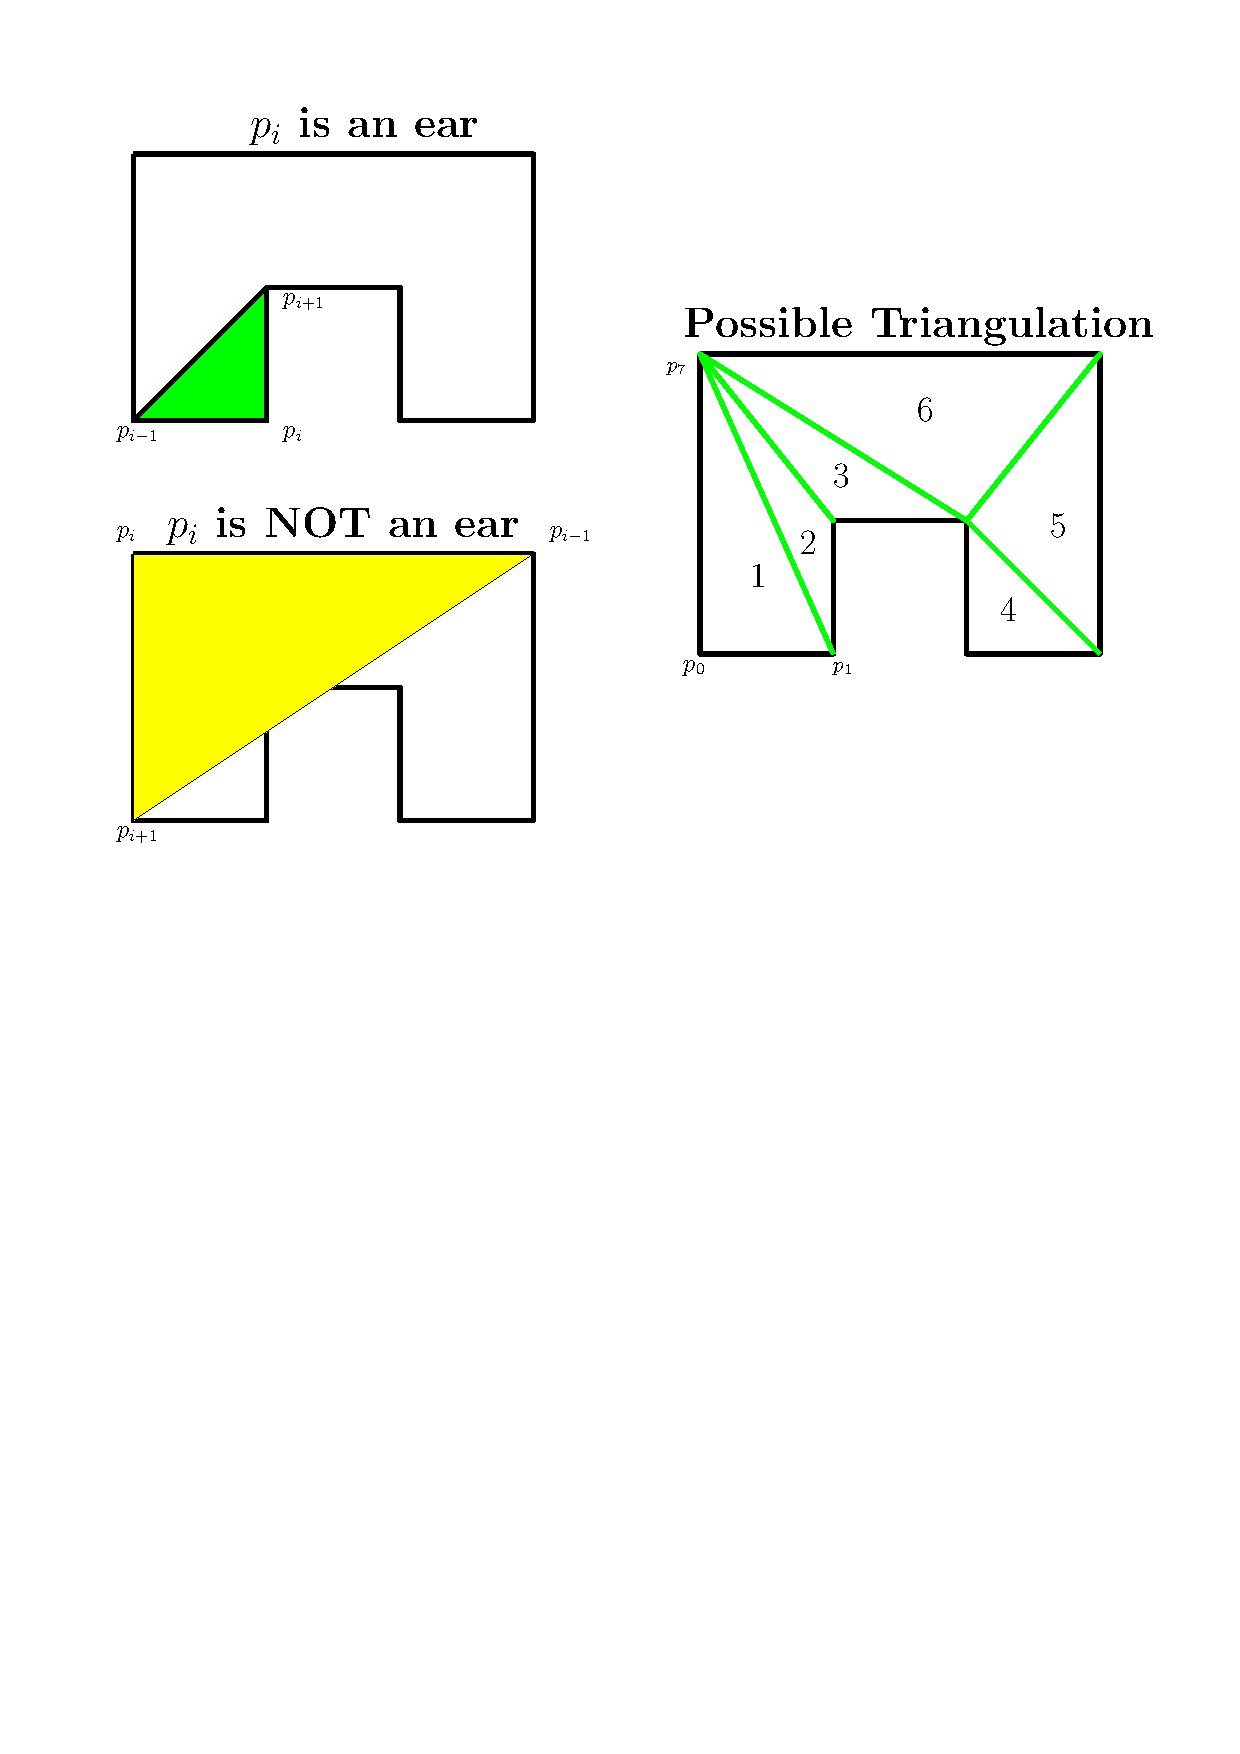
\includegraphics[width=.7\textwidth]{ear_slicing}
    \caption{Example of an ear and ear slicing result}
    \label{fig:ear_slicing}
\end{figure}

\subsection{Constructing roads and surface areas}
We like to use data from OpenStreetMap to construct models of roads, rivers, lakes and other types of surface area. Like described in chapter \ref{chap:OpenDataSets}, a Way in OpenStreetMap describes the position and area of a specific element. Most of Ways also contains a tag. We can use this tag to determine what kind of area the way describes, for example the type of land, water, type of road. If the type is defined in our system, then the system can take the appropriate measures to convert the way into the correct element and apply the corresponding texture. Furthermore, ways can contain meta-information. For example, roads may contain information about the number of lanes. We can use this to approximate the width of a road. For every lane 2.5 meter is used.

\section{System Design}
\label{sec:SystemDesign}
The system is divided in three parts. The first part pre-processes all the data, to filter only data that is needed. For example it can filter only data that is in Eindhoven and remove any unneeded metadata. The second step is the Tree building application. The tree-builder uses the pre-processed data and generates the complete tree with all the models. The final part of the application uses the tree and the models to give visualization to the user.

\section{Algorithms}
\label{sec:Algorithms}
\subsection{HLOD}
\label{subsec:HLOD}
A way to render more data while still getting a good quality on screen, a quad tree data structure like the one used by Davis \cite{Davis} is used. The root of the tree is node that covers the complete dataset. A child of a node covers one quarter of the data set presented its parent.

A child node is created by geometrically splitting up the parent in four parts. This process is executed recursively until the triangle count of the data within the child node is below a specified threshold. The triangle count is the total number triangles needed to render all the models which are present within the node. When all the data models for all the children of a node have been generated, then this node will contain simplified versions of all the data models of its children.

Data models are simplified with the following algorithm. Of all the models within the node, the model which contains the two closest consecutive points is taken. These two closest consecutive points are average together to create one new point. This is done until the triangle count is below the specified threshold.

To addresses the problem what has to be rendered, the node manager is used. The node manager determines which nodes have to be loaded and rendered on screen. This is done by replacing nodes which is currently being used by its children or by its parent. We devised an algorithm that determines which node has to replace which node. By using tree traversal it finds all the maximal nodes which need to be loaded into main memory. This is done by checking whether the error assigned to a node as metadata meets the current distance to that node. If this node has to be loaded, and it isn’t loaded yet, it checks for its entire sub-tree which nodes are currently loaded. For every loaded node in its sub-tree it unloads the nodes. If the current node does not need to be loaded, while it is loaded it will also be unloaded. This way the node manager makes sure all the models will be loaded with the appropriate level of detail.


\subsection{Complex polygons}
\label{subsec:ComplexPolygons}
The OSM data is built out of GPS recordings and these recordings have a lot of noise. The noise has the possibility of creating complex polygons in the OSM data. A complex polygon is polygon that contains an self-intersecting edge. In our OSM data set we have detected multiple complex polygons. This is a problem because the ear-clipping algorithm can only be used for simple polygons. A simple polygon is a polygon that does not contain any self-intersecting edges. The detection for complex polygons is a naïve algorithm. If two non-consecutive line-segments intersect, then the polygon is complex.

To generate a set of simple polygons from a complex polygon, the algorithm has to find two line-segments that intersect. The point at which two edges intersect, two new polygons can be generated. These two new polygons can still be a complex polygon, so the algorithm has to be recursively called on these new polygons. If the input polygon is already simple, then it simply returns the input polygon.

\section{Motivation of choices made}
\label{sec:MotivationOfChoicesMade}
\subsection{Simple polygon test}
\label{subsec:SimplePolygonTest}
Testing if a polygon is simple is done in a naïve way, a faster method is for example the Bentley-Ottmann algorithm \cite{Bentley79}. This algorithm has a running time of $O(\frac{n^2}{\log{n}})$, which is faster that our naïve way with running time $O(n^2)$. We choose the naïve way, since the polygons in the data set are not very large. The largest polygon in the data set containing only Eindhoven had 60 points. Also the time in which we had to develop the application demanded that we used an algorithm that was relative simple to implement.

\subsection{Simple triangulation}
\label{subsec:SimpleTriangulation}
The ear slicing algorithm implemented also has a running time of $O(n^2)$. There also exist algorithms which can triangulate a polygon in $O(n\log(n))$ and $O(n)$ time. These algorithms are however also more complex to implement. And just like for the simple polygon test, our dataset only contains relatively small polygon, therefore longer running times do not form a great constraint.
